%!TEX root = ..\..\main.tex
\chapter{Mixture Likelihoods}
\label{Ch: Mixture Likelihoods}

\lhead{Chapter \ref{Ch: Mixture Likelihoods}. \emph{Mixture Likelihoods}}

We are given a random sample $X_1,X_2,\dots,X_n$ from an unknown distribution. We wish to estimate the density of this distribution using a mixture density. Let $f_\theta(x)$ be a probability density with parameter $\theta \in \mathbb{R}$. The \emph{mixture density} corresponding to the \emph{mixing distribution} $Q$ is given by
\begin{equation}
	f_Q(x) = \int_{-\infty}^{\infty} f_\theta(x) \intd Q(\theta).
	\label{eq:mixturedefinition}
\end{equation}

Our aim is to find a distribution $Q$ that maximizes the likelihood
\begin{equation}
	l(Q) = \prod_{i = 1}^n f_Q(X_i)
	\label{eq:nonloglikelihood}
\end{equation}
or equivalently the log likelihood
\begin{equation}
	L(Q) = \sum_{i = 1}^n \log(f_Q(X_i)).
	\label{eq:likelihood}
\end{equation}

\section{The Geometry of Mixture Likelihoods}
\label{sec:mixturelikelihoods:geometrical}
	In \cite{Lindsay1983-tf}, the mixture likelihood problem was looked at from a geometrical perspective. This was used to show that, under weak conditions, \eqref{eq:likelihood} can be maximized by a discrete $Q$ with no more than $n$ point masses. Here we will summarise the geometrical approach and restate this result.

	Let $U$ be the set of all $\vect{u} = (u_1,\dots,u_n)$ that satisfy the constraint
	\begin{align}
	u_i &= f_Q(X_i)	&& i = 1,\dots,n
	\label{eq:likelihoodconstraint}
	\end{align}
	for some distribution $Q$. Then maximizing \eqref{eq:likelihood} is equivalent to maximizing
	\begin{equation}
	M(\vect{u}) = \sum_{i=1}^n \log(u_i)
	\label{eq:transformedlikelihood}
	\end{equation}
	over $\vect{u} \in U$. That is,
	\begin{equation}
	\max_Q L(Q)  = \max_{\vect{u} \in U} M(\vect{u})
	\end{equation}
	and any $\vect{u} \in U$ that maximizes $M(\vect{u})$ satisfies \eqref{eq:likelihoodconstraint} for a $Q$ that maximizes $L(Q)$. We say both that $\vect{u}$ and $Q$ maximize the likelihood. This is essentially a change of variables that moves the original optimization problem over the space of distributions to an optimization problem in $\mathbb{R}^n$. 

	Our aim is now to get a better picture of what our set of feasible points, $U$, looks like. We introduce the following vector
	\begin{equation}
	\vect{f}(\theta) = (f_\theta(X_1),f_\theta(X_2),\dots,f_\theta(X_n))
	\end{equation}
	which we call the \emph{component likelihood vector}. We define
	\begin{equation}
	\Gamma = \left\{ \vect{f}(\theta) : \theta \in \mathbb{R} \right\}
	\end{equation}
	to be the set of all possible values of the component likelihood vector.

	Now from \eqref{eq:mixturedefinition},
	\begin{equation}
	f_Q(X_i) = \int_{-\infty}^{\infty} f_\theta(X_i) \intd Q(\theta)
	\end{equation}
	and in the case that $Q$ is discrete with point masses $p_1,\dots,p_m$ at locations $\theta_1,\dots,\theta_m$ this becomes
	\begin{equation}
	f_Q(X_i) = \sum_{j = 1}^m p_j f_{\theta_j}(X_i).
	\end{equation}
	Hence any convex combination of the component likelihood vector
	\begin{align}
	\vect{u} &= \sum_{j = 1}^m p_j \vect{f}(\theta_j), && \sum_{j=1}^m p_j = 1
	\end{align}
	satisfies \eqref{eq:likelihoodconstraint} for the distribution $Q$ that puts masses $p_1,\dots,p_m$ at locations $\theta_1,\dots,\theta_m$. Since $\conv(\Gamma)$ is precisely the set of all convex combinations of points in $\Gamma$ we must have that $\conv(\Gamma) \subseteq U$. If we make the additional assumption that $\Gamma$ is compact then $\conv(\Gamma) = U$ \cite{Phelps2001-ba}, Proposition 1.2). 

	We note that we are maximizing a concave function \eqref{eq:transformedlikelihood} over a convex set, $\conv(\Gamma)$, and so the optimal point must lie on the boundary of $\conv(\Gamma)$. From Carathéodory's theorem \cite{Roberts1973-cx}, we can write this as the convex combination of no more than $n$ points in $\Gamma$. This gives us the following theorem from \cite{Lindsay1983-tf}.

	\begin{theorem}
		If $\Gamma$ is compact then there exists a unique point on the boundary of $\conv(\Gamma)$ which maximizes the likelihood. This point corresponds to a distribution $Q$ which maximizes the likelihood and that has no more than $n$ point masses.
		\label{thm:LindsayGamma}
	\end{theorem}


\section{Example}
\label{sec:mixturelikelihoods:example}
	The following example illustrates the geometrical approach given above. We consider the case where $n = 2$. Our sample is made up of two points, $X_1 = 1$ and $X_2 = 2$. We define
	\begin{equation}
	f_\theta(x) = \frac{1}{0.45 \sqrt{2 \pi}} \exp\left(-\frac{(x-\theta)^2}{2\cdot 0.45^2}\right)
	\end{equation}
	(i.e. a normal density with mean $\theta$ and variance $\sigma^2 = 0.45^2$) to be our component density.
	We trace out the set $\Gamma$ in Figure \ref{fig:TracingGamma}. 

	\begin{figure}[ht]
		\centering
		\begin{minipage}[b]{0.3\linewidth}
			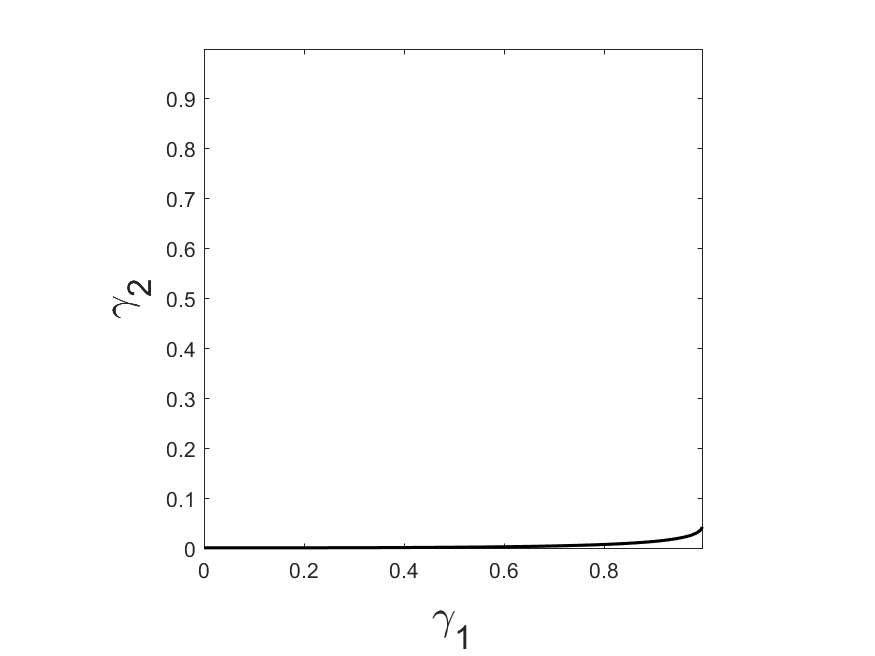
\includegraphics[width=\textwidth]{MixtureLikelihoods/GammaTrace01}
		\end{minipage}
		\begin{minipage}[b]{0.3\linewidth}
			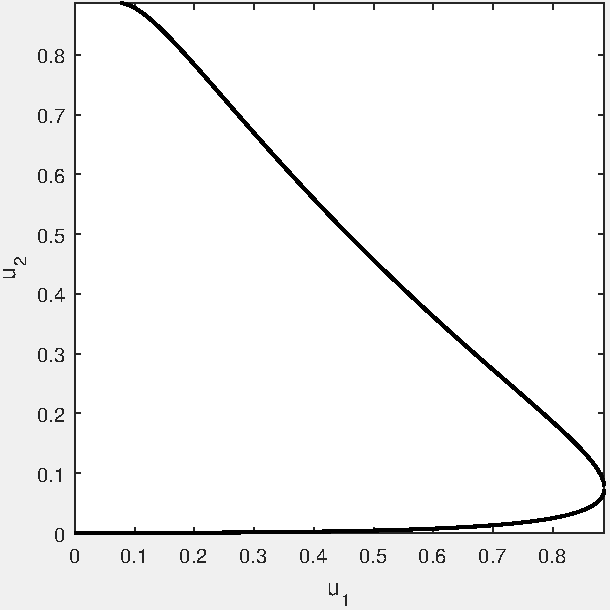
\includegraphics[width=\textwidth]{MixtureLikelihoods/GammaTrace02}
		\end{minipage}
		\begin{minipage}[b]{0.3\linewidth}
			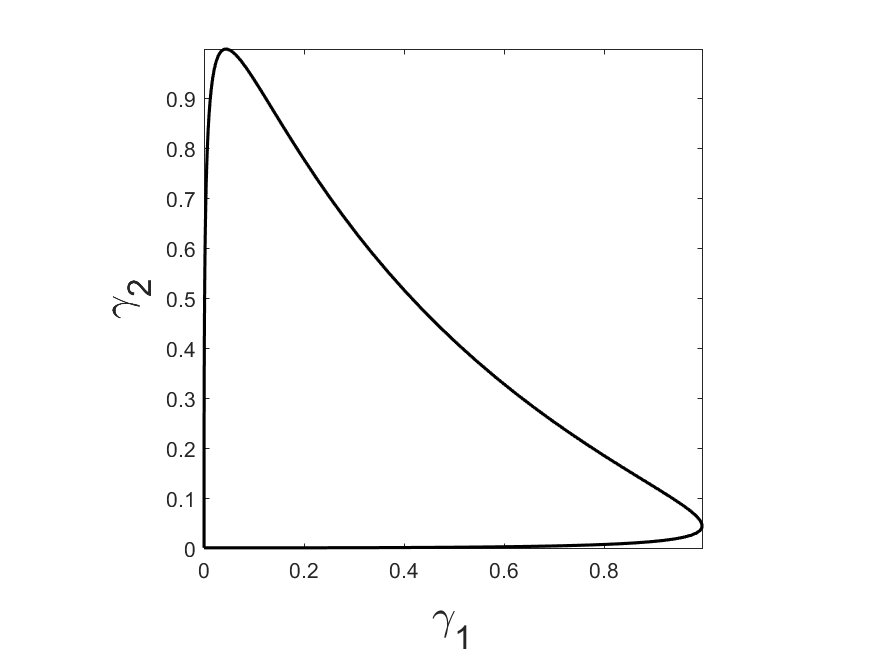
\includegraphics[width=\textwidth]{MixtureLikelihoods/GammaTrace03}
		\end{minipage}
		\begin{minipage}[b]{0.3\linewidth}
			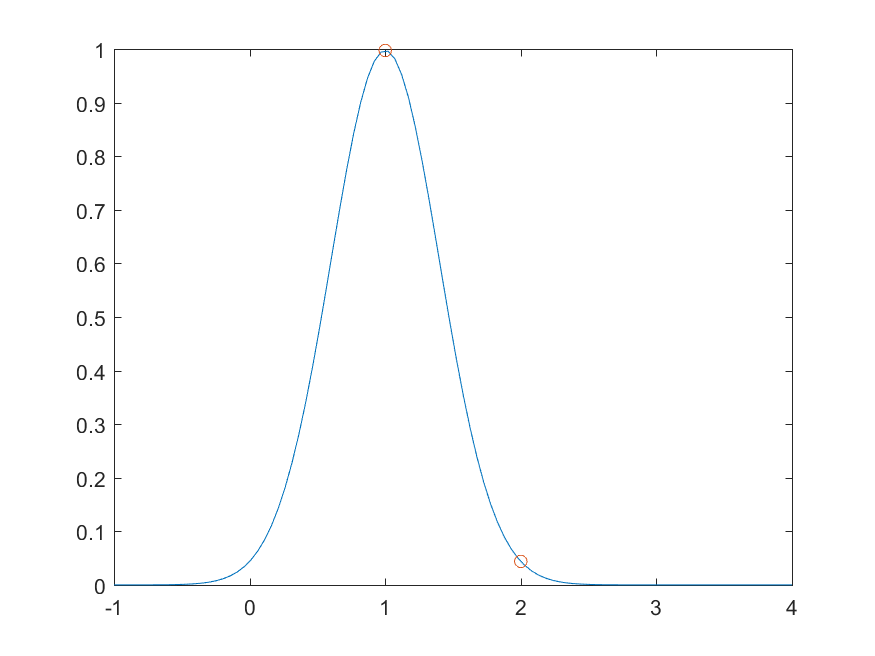
\includegraphics[width=\textwidth]{MixtureLikelihoods/GammaTraceDensity01}
			\subcaption{$\theta = 1$}
		\end{minipage}
		\begin{minipage}[b]{0.3\linewidth}
			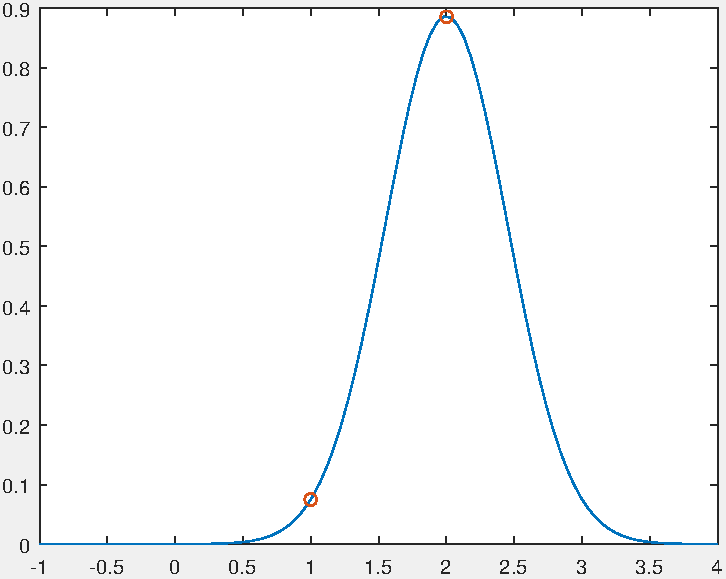
\includegraphics[width=\textwidth]{MixtureLikelihoods/GammaTraceDensity02}
			\subcaption{$\theta = 2$}
		\end{minipage}
		\begin{minipage}[b]{0.3\linewidth}
			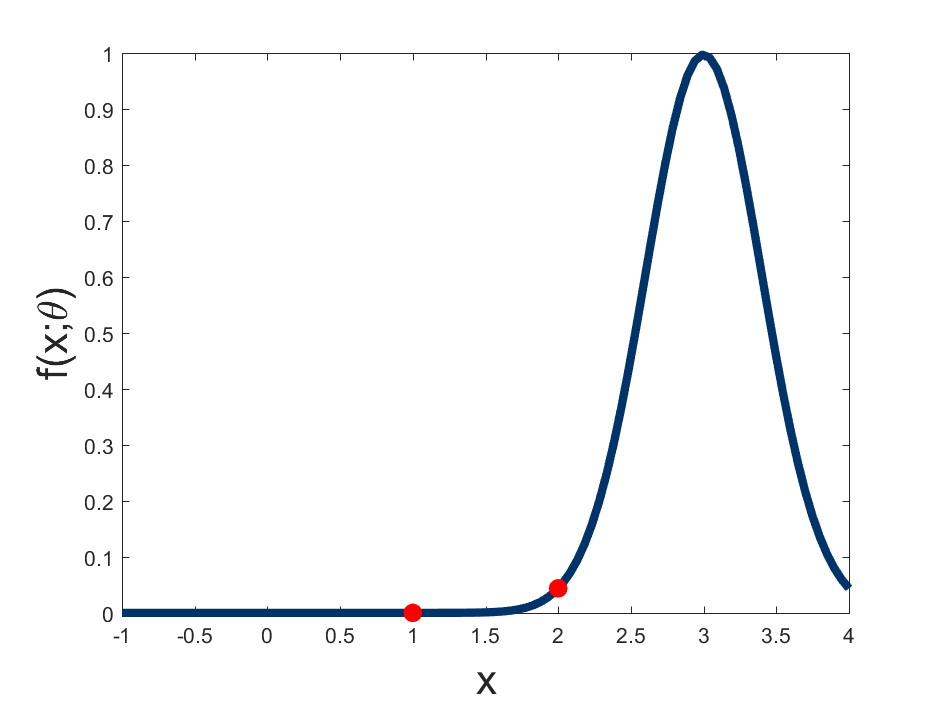
\includegraphics[width=\textwidth]{MixtureLikelihoods/GammaTraceDensity03}
			\subcaption{$\theta = 3$}
		\end{minipage}
		\caption{The blue density is $f_\theta$ for $\theta = 1,2,3$. Each value of $\theta$ contributes a point to $\Gamma$ whose coordinates are given by $(f_\theta(X_1),f_\theta(X_2))$ (represented by the red circles). As we increase $\theta$ from $-\infty$ to $\infty$ we trace out more of $\Gamma$ (shown above).}\label{fig:TracingGamma}
	\end{figure}

	Note that while $\Gamma$ is bounded, it is not closed (it does not contain the limit point $(0,0)$), and so $\Gamma$ is not compact (as required by Theorem \ref{thm:LindsayGamma}). In fact, any positive density whose support is the whole real line will not contain the limit point $\vect{0}$ (where $\vect{0}$ represents the zero vector in $\mathbb{R}^n$). However, since $\vect{0}$ is clearly not going to be a part of a maximizing mixture, we are safe to apply Theorem \ref{thm:LindsayGamma} if $\Gamma \cup \{ \vect{0} \}$ is compact.

	%and so we will provide a slightly more general form of Theorem \ref{thm:LindsayGamma}.
	%\begin{theorem}
	%	Write $\vect{0}$ for the zero vector in $\mathbb{R}^n$. If $\Gamma \cup \{ \vect{0} \}$ is compact then there exists a unique point on the boundary of $\conv(\Gamma)$ which maximizes the likelihood. This point corresponds to a distribution $Q$ which maximizes the likelihood and that has no more than $n$ point masses.
	%\end{theorem}
	%\begin{proof}
	%	We need to show that $\vect{0}$ does not appear in the maximizing mixture. Clearly, $\vect{0}$ is not going to be a maximizing point.
	%\end{proof}

	We trace the boundary of $\conv(\Gamma)$ in Figure \ref{fig:GammaSol} along with a heat map of the objective function \eqref{eq:transformedlikelihood}.
	\begin{figure}[ht]
		\centering
		\begin{minipage}{0.4\textwidth}
			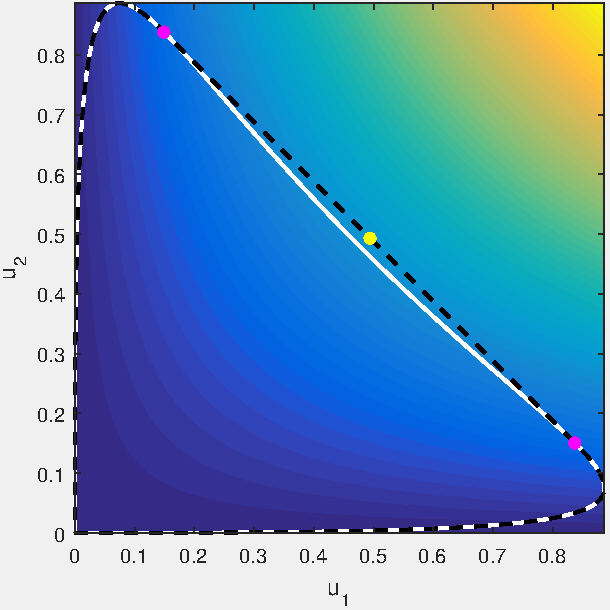
\includegraphics[width = \textwidth]{MixtureLikelihoods/GammaOptimHullSol}
			\subcaption{}\label{fig:GammaSol:subfig:Gamma}
		\end{minipage}
		\begin{minipage}{0.5\textwidth}
			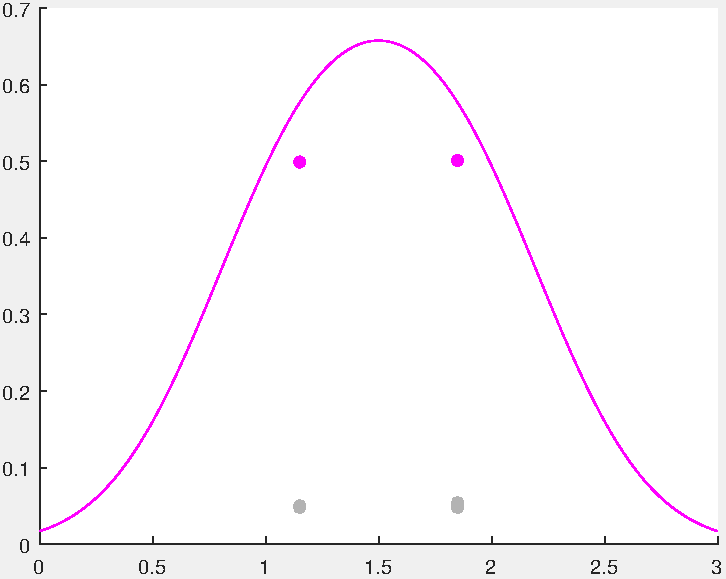
\includegraphics[width = \textwidth]{MixtureLikelihoods/MixingSolSigma045}				\subcaption{}\label{fig:GammaSol:subfig:Density}
		\end{minipage}
		\caption{In (\subref{fig:GammaSol:subfig:Gamma}), the boundary of $\conv(\Gamma)$ is shown as a dashed black line, $\Gamma$ is the white curve, the heat map  shows the objective function (likelihood increases from blue to yellow) and the yellow point is the maximizing point which can be written as the convex combination of the two magenta points. These two magenta points correspond to the two probability masses in the maximizing mixing distribution (\subref{fig:GammaSol:subfig:Density}).}
		\label{fig:GammaSol}
	\end{figure}
	The optimal point is on the boundary of $\conv(\Gamma)$ as expected and it can be written as the  $p_1 \vect{f}(\theta_1) + p_2 \vect{f}(\theta_2)$ (where $p_1 + p_2 =1 $). These two points correspond to the two probability masses in the maximizing mixture distribution shown in Figure \ref{fig:GammaSol:subfig:Density}. These masses are located at $\theta_1$ and $\theta_2$ with weights $p_1$ and $p_2$.

	\subsection{The effect of variance}
	In Figure \ref{fig:variance of ftheta}, we still use a normal density with mean $\theta$ as $f_\theta$ but we observe the effect that varying the variance, $\sigma^2$, has on the shape of $\Gamma$. We note that once $\sigma$ is large enough, the optimal point lies on $\Gamma$ and so only one point is needed in the maximum likelihood mixing distribution.
	\begin{figure}[ht]
		\centering
		\begin{minipage}{0.3\textwidth}
			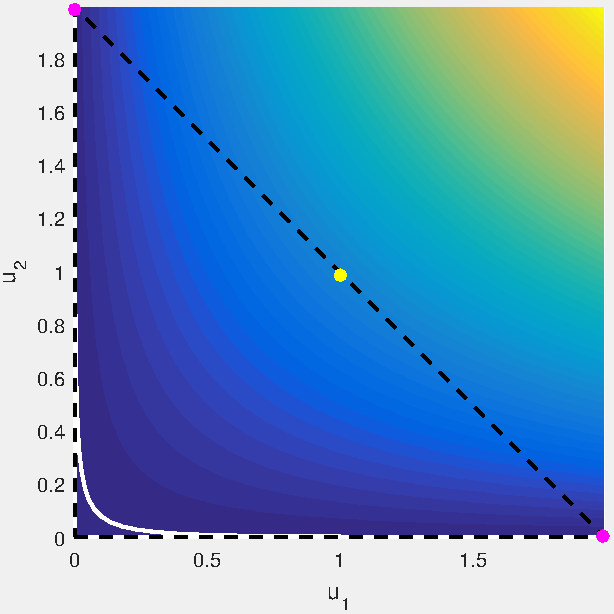
\includegraphics[width = \textwidth]{MixtureLikelihoods/GammaSigma02}
		\end{minipage}
		\begin{minipage}{0.3\textwidth}
			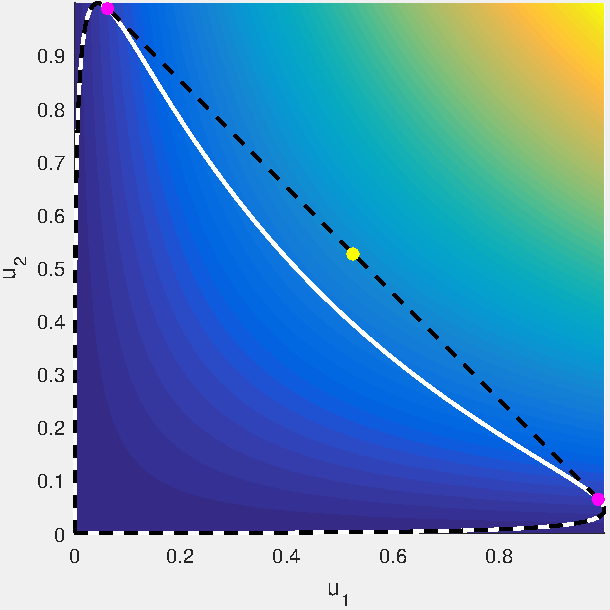
\includegraphics[width = \textwidth]{MixtureLikelihoods/GammaSigma04}
		\end{minipage}
		\begin{minipage}{0.3\textwidth}
			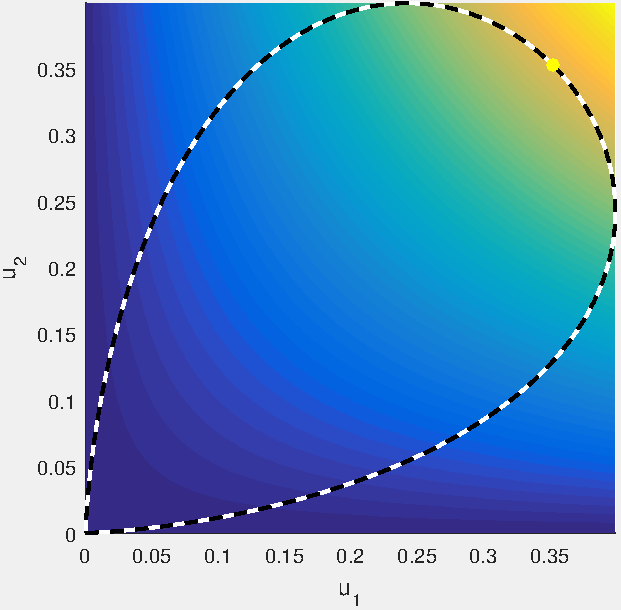
\includegraphics[width = \textwidth]{MixtureLikelihoods/GammaSigma1}
		\end{minipage}
		\begin{minipage}{0.3\textwidth}
			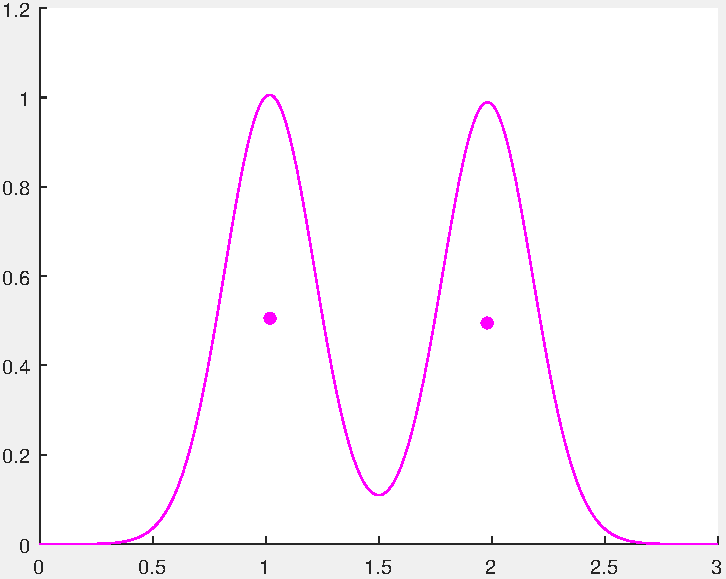
\includegraphics[width = \textwidth]{MixtureLikelihoods/MixingSolSigma02}
			\subcaption{$\sigma = 0.2$}
		\end{minipage}
		\begin{minipage}{0.3\textwidth}
			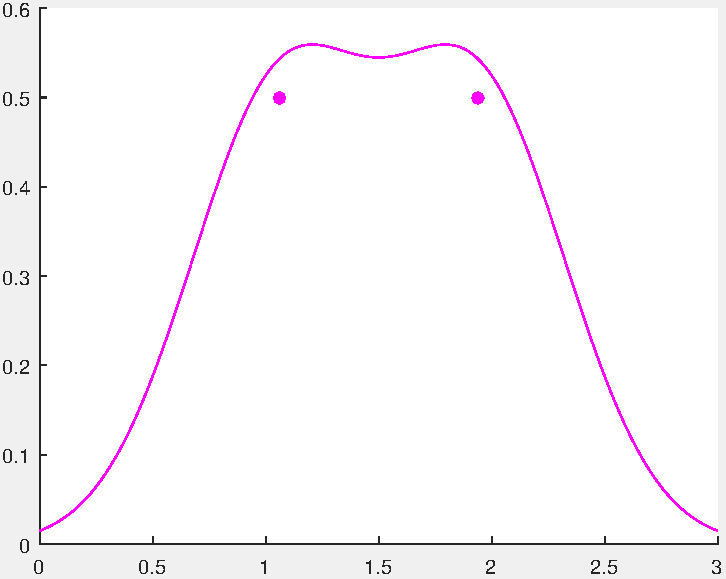
\includegraphics[width = \textwidth]{MixtureLikelihoods/MixingSolSigma04}
			\subcaption{$\sigma = 0.4$}
		\end{minipage}
		\begin{minipage}{0.3\textwidth}
			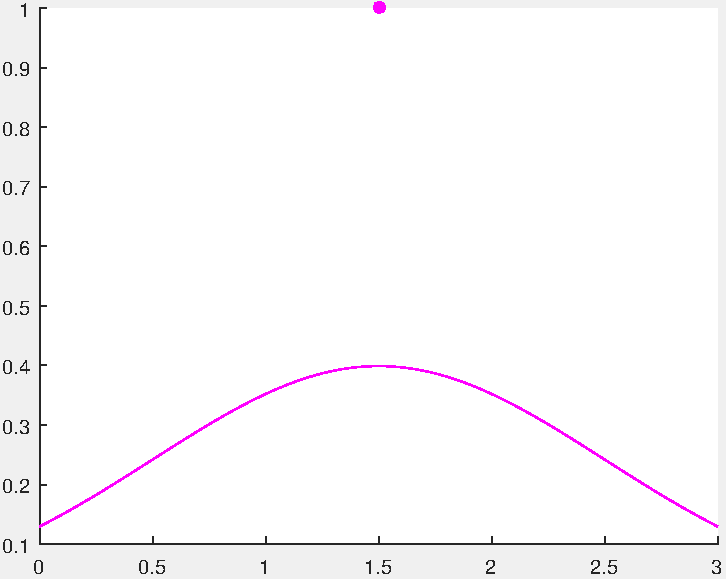
\includegraphics[width = \textwidth]{MixtureLikelihoods/MixingSolSigma1}
			\subcaption{$\sigma = 1$}
		\end{minipage}
		\caption{The maximum likelihood density for two points $X_1 = 1$ and $X_2 = 2$ where the component density, $f_\theta$, is a normal density with mean $\theta$ and variance $\sigma^2$. The variance is increased from left to right.}
		\label{fig:variance of ftheta}
	\end{figure}


	%\subsection{Critical value of $\sigma$}
		Figure \ref{fig:variance of ftheta} suggests that, for a fixed $X_1$ and $X_2$, there is a critical value of $\sigma$ at which the maximum likelihood mixing distribution, $Q$, goes from having two probability masses to having just one.
		
		\begin{theorem}
			If we have a sample with two points, $X_1$ and $X_2$, and we are finding the maximum likelihood mixture density for these points with 
			$$f_\theta(x) = \frac{1}{\sigma \sqrt{2\pi}} e^{-\frac{(x-\theta)^2}{2\sigma^2}}$$
			then a maximizing mixture distribution with only one probability mass exists if and only if
			$$|X_1 - X_2| \leq 2 \sigma$$
			\label{thm:distancebetweentwopoints}
		\end{theorem}
		We present two different proofs for this theorem.
		\begin{proof}[Proof 1]
			By stuff, if $|X_1 - X_2| \leq 2 \sigma$ then $\Gamma$ is convex and so optimal point must lie on $\Gamma$ and hence the corresponding maximizing mixture distribution has only one probability mass.
			If $|X_1 - X_2| > 2\sigma$ then just look at the picture... it's obvious... why do I have to make this so rigorous!?
		\end{proof}
		\begin{proof}[Proof 2]
			blah
		\end{proof}
	
\section{Differentiation of the log likelihood}
	This is from \cite{Lindsay1983-tf} but adapted for our context. We define the directional derivative of the likelihood from $Q_0$ to $Q_1$ to be
	$$\Phi(Q_1,Q_0) = \lim_{\epsilon \rightarrow 0} \epsilon^{-1} \left( L((1-\epsilon)Q_0 + \epsilon Q_1;\vect{y}) - L(Q_0;\vect{y}) \right).$$
	\begin{theorem}[Thm 4.1 from \cite{Lindsay1983-tf}]
		\label{thm:thm4point1}
		Let $\delta_\theta$ be the distribution that concentrates all of its mass at $\theta$. Then for any $Q$
		$$\sup_\theta \Phi(\delta_\theta,Q) \geq 0$$
		with equality if and only if $Q$ maximizes \eqref{eq:likelihood}.
	\end{theorem}

	\subsection{A strictly increasing sequence}
	%	We define a sequence $\{Q_j\}_{j=1}^n$ of discrete mixing distributions where
	%	$$Q_j = \argmax_{Q \text{ with no more than $j$ points of support}} L(Q;\vect{y})$$
	%	We define $\jmax = \argmax_j L(Q_j;\vect{y})$.

	Let $S_j$ be the set of all discrete mixing distributions with at most $j$ points of support. Consider the sequence $\{\alpha_j\}_{j=1}^n$ with
	\begin{equation}
	\alpha_j = \sup_{Q\in S_j} L(Q;\vect{y}).
	\label{eq:sequence}
	\end{equation}
	We know that this sequence must contain the maximum likelihood as there always exists a maximizing mixing distribution $\hat{Q}$ with no more than $n$ points of support. Let $\jmax$ be the smallest integer such that $\alpha_\jmax = L(\hat{Q})$. Clearly, $\alpha_\jmax = \alpha_{\jmax+1} = \dots = \alpha_n$.

	\begin{lemma} \label{lem:sequencestrictlyincreasing}
		The sequence $\{ \alpha_j\}_{j=1}^{\jmax}$ is strictly increasing.
	\end{lemma}
	\begin{proof}	
		
		It is not immediately clear whether or not we can replace the supremum in \eqref{eq:sequence} with a maximum. I'm pretty sure we can (I can't see how we could have a sequence of distributions in $S_j$ that converges to a distribution not in $S_j$) so let's just assume we can for now.
		
		Let $j < \jmax$ and choose some $Q_j \in S_j$ such that $\alpha_j = L(Q_j;\vect{y})$. From Theorem \ref{thm:thm4point1}, there exists some $\theta_0$ such that $\Phi(\delta_{\theta_0},Q_j) > 0$. Then for some $0<\epsilon <1$, $Q^* = (1-\epsilon)Q_j + \epsilon \delta_{\theta_0}$ satisfies $L(Q^*;\vect{y}) > L(Q_j;\vect{y})$. Now $Q^*$ has points of support at $\theta_0$ and at the points of support of $Q_j$. Hence $Q^*$ has no more than $j+1$ points of support. However, $Q^*$ must have more than $j$ points of support since $L(Q^*;\vect{y}) > \alpha_j$. So $Q^*$ has $j+1$ points of support and so $\alpha_{j+1} \geq L(Q^*;\vect{y}) > \alpha_j$.
		%This tells us that $\{\alpha_j\}_{j=1}^n$ is strictly increasing up to $\alpha_\jmax$ and is then constant.
	\end{proof}

\section{Additional Theorems about number of points}
	\begin{theorem}
		Given a sample $X_1,X_2,\dots,X_n$, define
		$$\epsilon = \min_{i \neq j}|X_i - X_j|.$$
		Define the density function
		$$f_\theta(x) = \begin{cases}
			1/\epsilon & \theta - \epsilon/2 < x < \theta + \epsilon/2\\
			0 &\text{otherwise.}
		\end{cases}$$
		Then there exists a discrete mixing distribution $Q$ with $n$ point masses that maximizes the likelihood
		$$\prod_{i = 1}^n \int_{-\infty}^{\infty} f_\theta(X_i) \intd Q(\theta)$$
	\end{theorem}
	\begin{proof}
		If $f_Q(X_i) = 0$ for any $i$ then $L(Q) = 0$. For any value of $\theta$, $f_\theta(x)$ is non-zero at no more than one $X_i$ and so $L(Q) > 0$ only for a $Q$ with at least $n$ point masses. By Theorem \ref{thm:LindsayGamma}, we need no more than $n$.
	\end{proof}
	\begin{theorem}
		Given a sample $X_1,X_2,\dots,X_n$, define
		$$E = \max_{i,j}|X_i - X_j|.$$
		Define the density function
		$$f_\theta(x) = \begin{cases}
		1/E & \theta - E/2 \leq x \leq \theta + E/2\\
		0 &\text{otherwise.}
		\end{cases}$$
		Then there exists a discrete mixing distribution $Q$ with 1 point mass that maximizes the likelihood
		$$L(Q) = \prod_{i = 1}^n \int_{-\infty}^{\infty} f_\theta(X_i) \intd Q(\theta)$$
	\end{theorem}
	\begin{proof}
		Consider the distribution $Q_0$ that puts a mass at $\theta_0 = (X_{max} - X_{min})/2$. The likelihood is $L(Q_0) = \left( \frac{1}{E} \right)^n$. Obviously the density at each $X_i$ is the maximum that it can possibly be and so $Q_0$ is a maximum likelihood mixing distribution.
	\end{proof}
	
	Remark: There is an important distinction when defining the density function as to whether you use $\leq$ or $<$. This feels a little strange.